\section{Exemples d'images provenant du RETIF}

\begin{figure}[H]
    \centering
    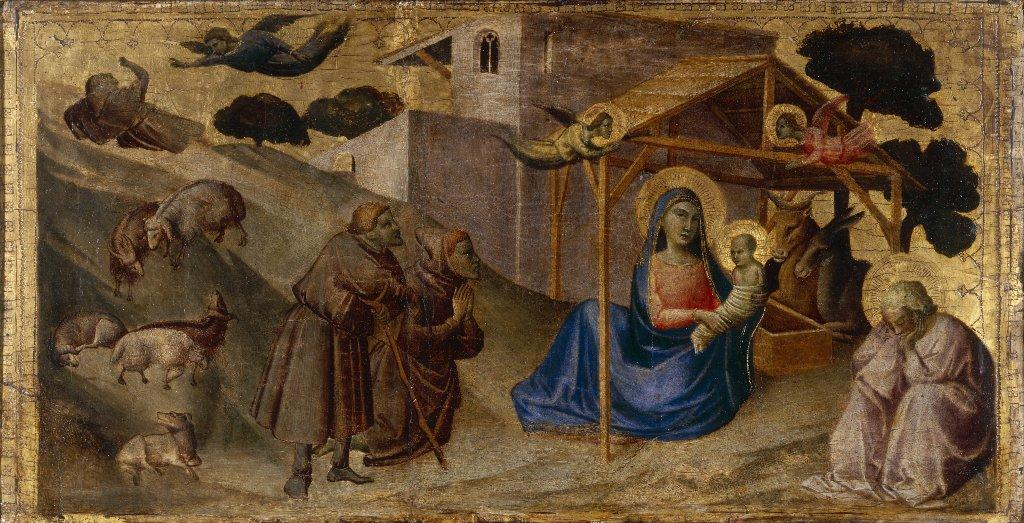
\includegraphics[width=1\textwidth]{annexes/figures/ptrGaddiAdoration.jpg}
    \caption{Taddeo Gaddi, \textit{L'Adoration des bergers}, vers 1330, tempéra sur bois, Dijon, Musée des Beaux-Arts, inv. 1470 © Musée des Beaux-Arts de Dijon}
    \label{fig:ptrGaddiAdoration}
\end{figure}


\begin{figure}[H]
    \centering
    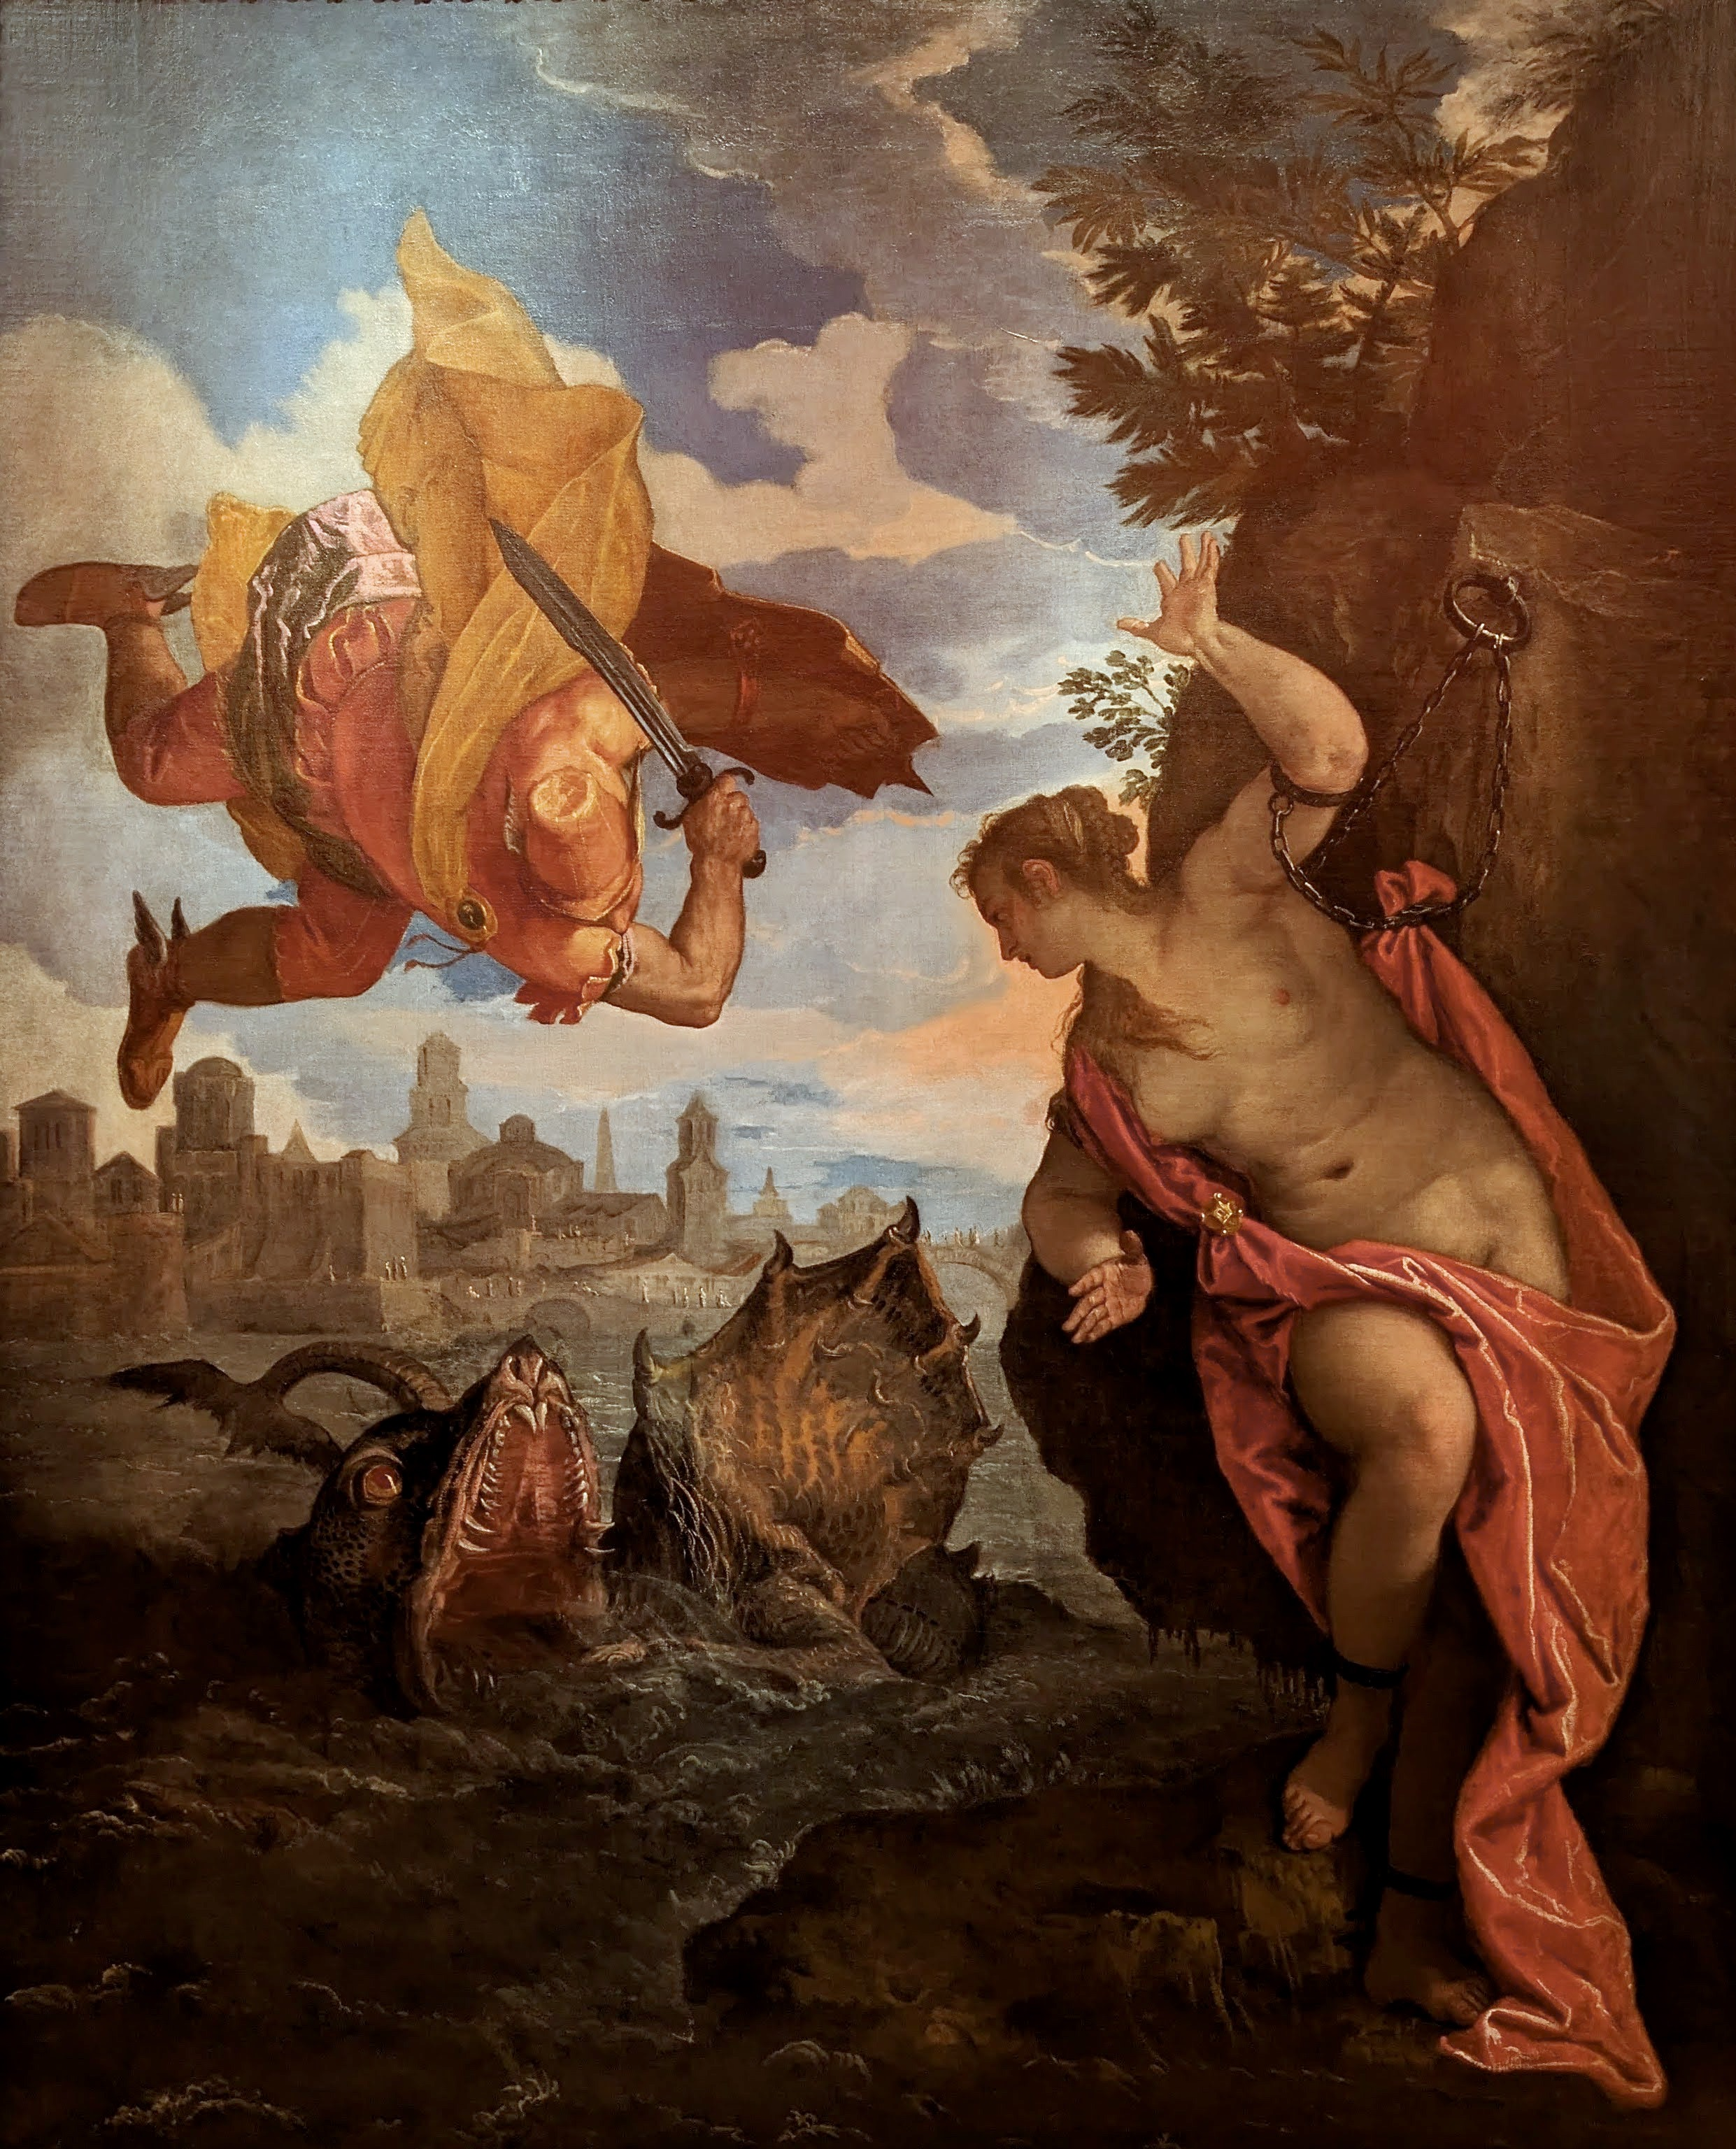
\includegraphics[height=0.4\textheight]{annexes/figures/ptrVeronesePersee.jpg}
    \caption{Paul Véronèse, \textit{Persée délivrant Andromède}, 1575-1580, peinture à l'huile sur toile, Rennes, Musée des Beaux-Arts de Rennes, inv. 801.1.1}
    \label{fig:ptrVeronesePersee}
\end{figure}

\begin{figure}[H]
    \centering
    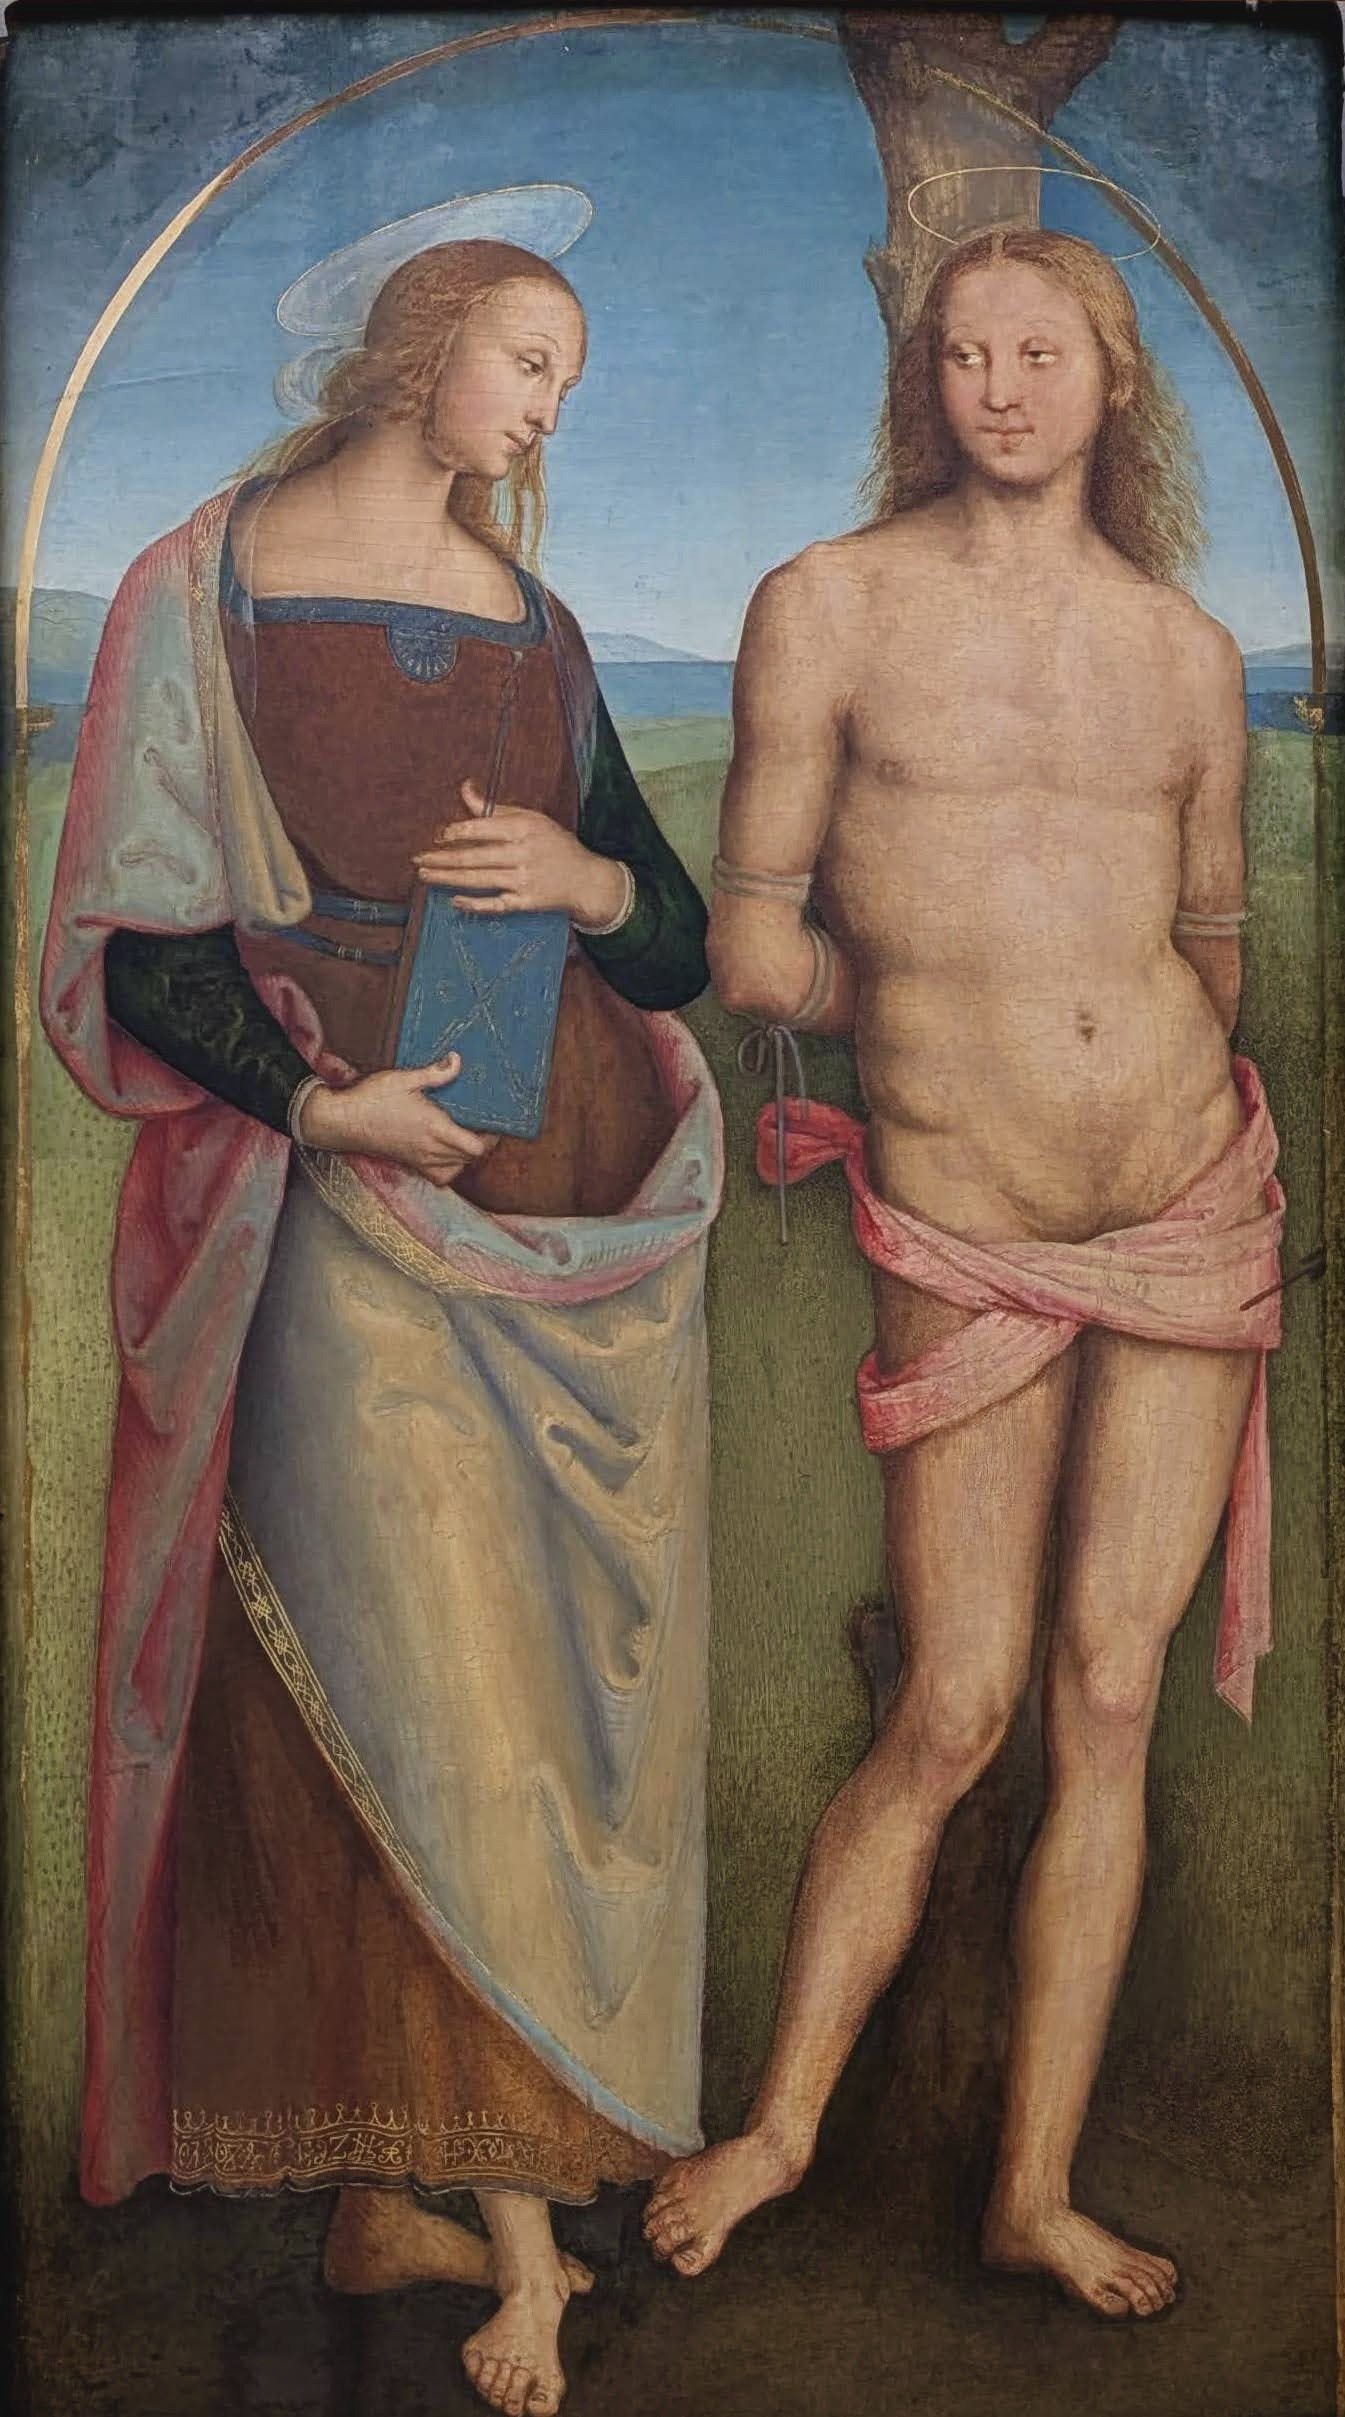
\includegraphics[height=0.4\textheight]{annexes/figures/ptrPeruginSaints.jpg}
    \caption{Pérugin, \textit{Saint Sébastien et sainte Apolline}, 1513 -1523, peinture à l'huile sur toile, Grenoble, Musée de Grenoble, inv. MG 48}
    \label{fig:ptrPeruginSaints}
\end{figure}

\begin{figure}[H]
    \centering
    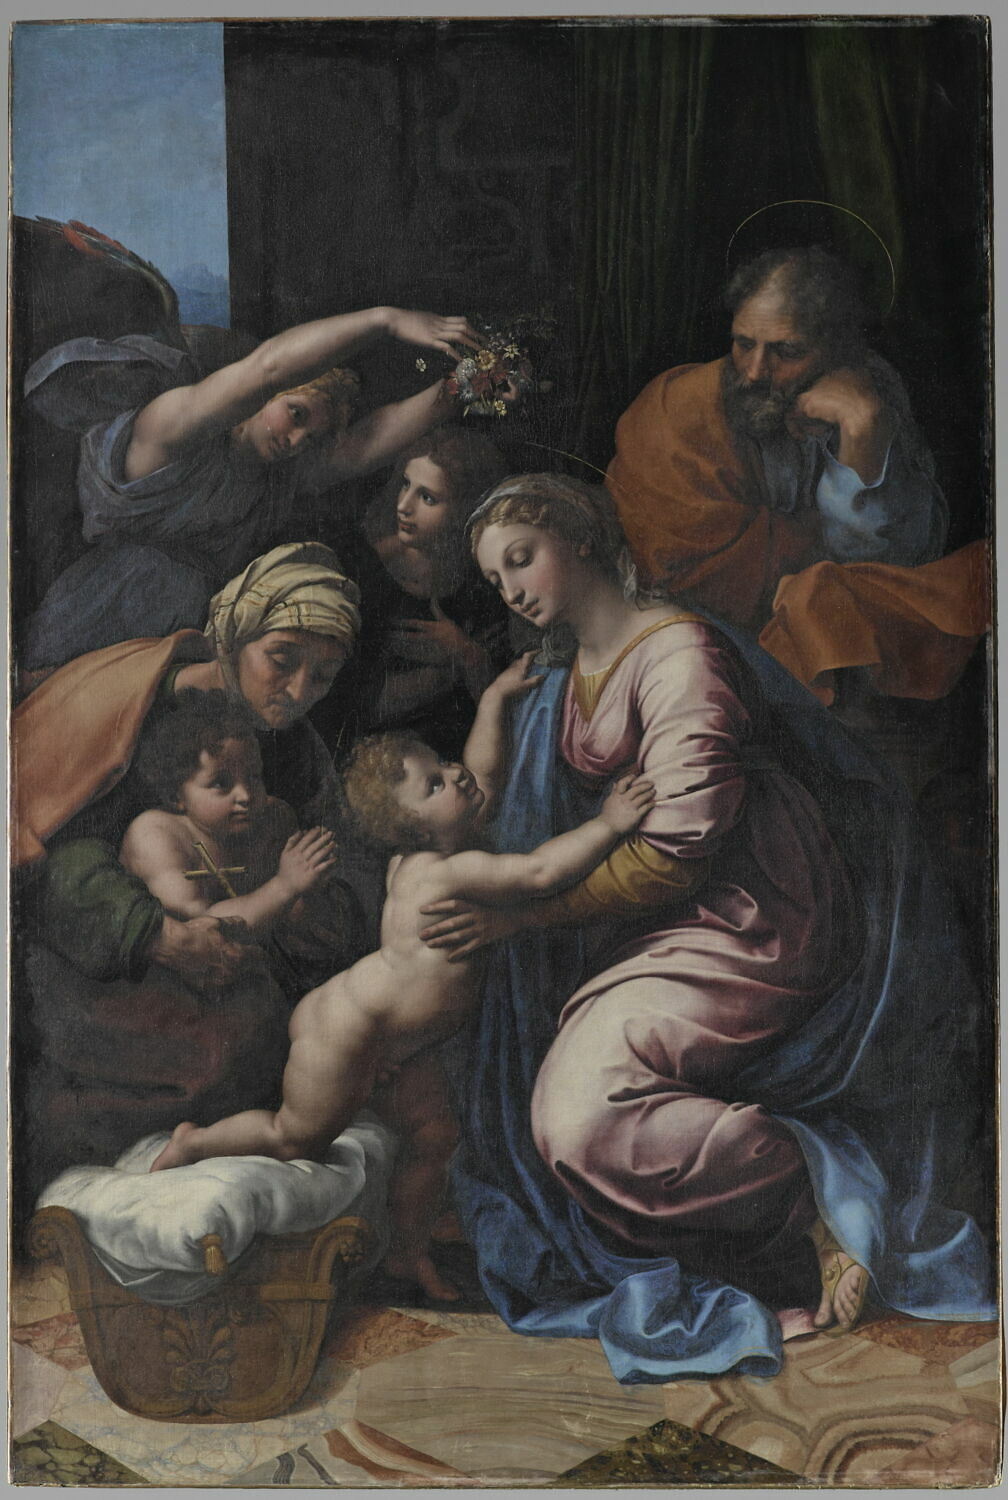
\includegraphics[height=0.4\textheight]{annexes/figures/ptrRaphaelSteFam.jpg}
    \caption{Raphaël, \textit{La Sainte Famille, dit La Grande Sainte Famille de François Ier}, 1518, peinture à l'huile sur toile, Paris, Musée du Louvre, INV 604 ; MR 432 © 2013 GrandPalaisRmn (musée du Louvre) / Adrien Didierjean}
    \label{fig:ptrRaphaelSteFam}
\end{figure}


\section{Exemples d'images inexploitables}

\begin{figure}[H]
    \centering
    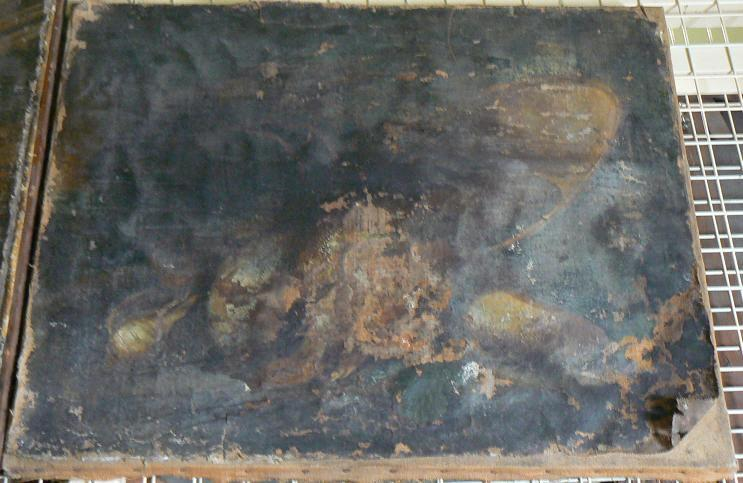
\includegraphics[height=0.3\textheight]{annexes/figures/ptrRecco.jpg}
    \caption{Giuseppe Recco \textit{Nature morte : poisson de mer et chaudron}, Musée des Beaux-Arts (Orléans), inv. 1173, Lien AGORHA : \\ \url{https://agorha.inha.fr/ark:/54721/d5fc162e-48a3-4508-9a6c-562fb76c1a1a}}
    \label{fig:ptrRecco}
\end{figure}


\begin{figure}[H]
    \centering
    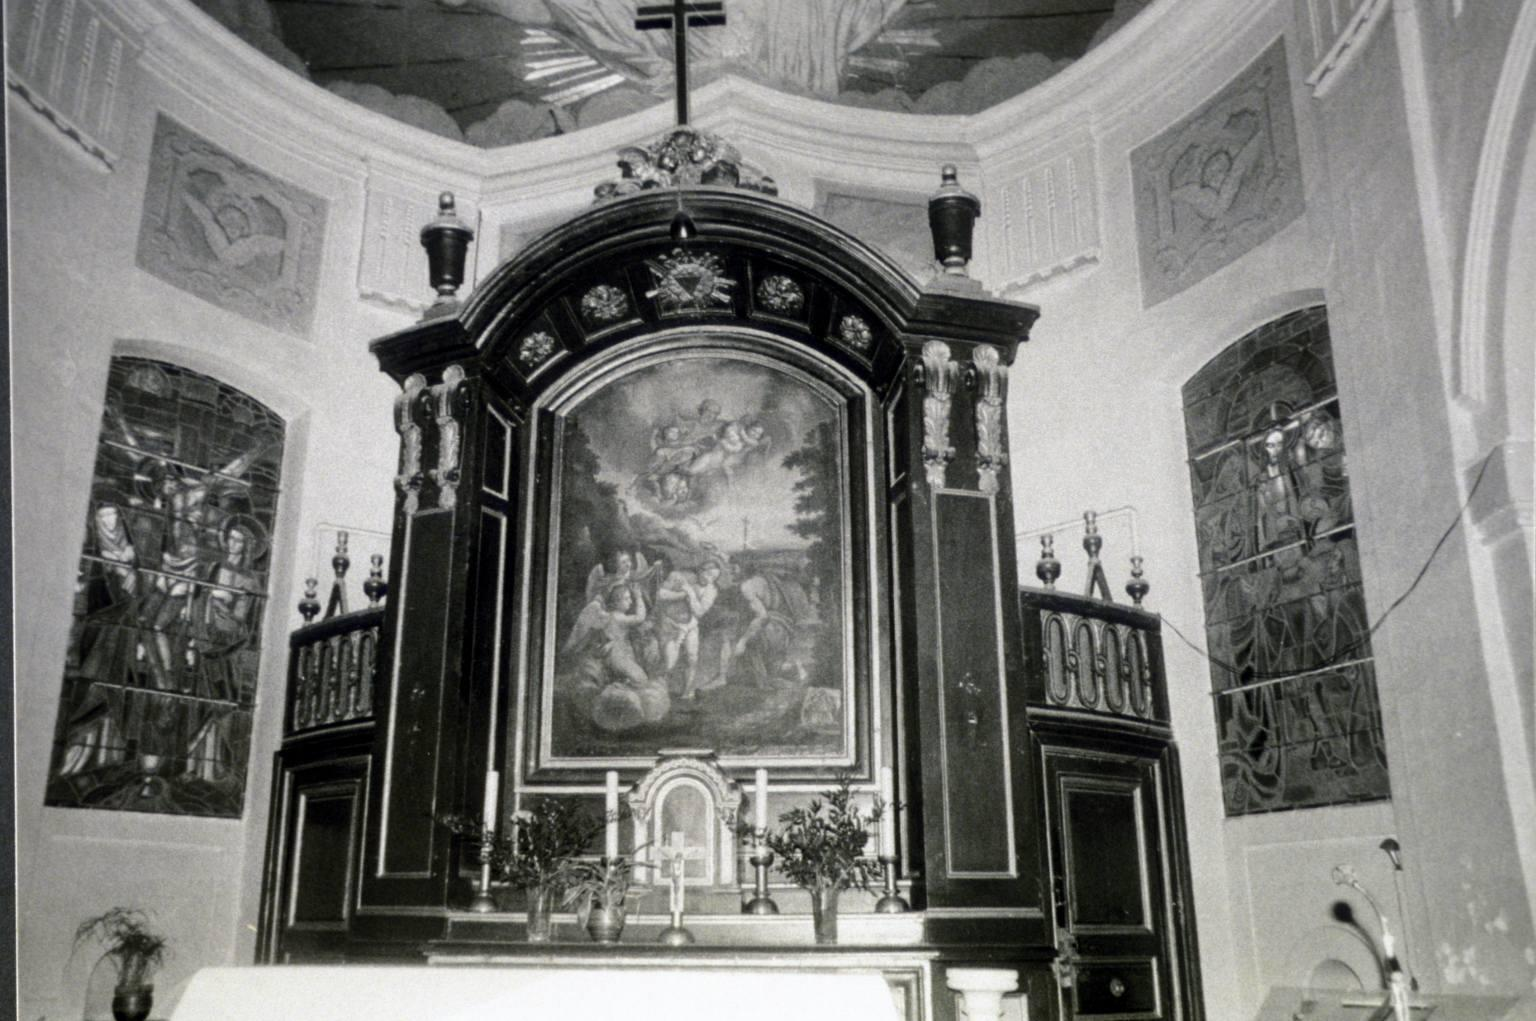
\includegraphics[height=0.4\textheight]{annexes/figures/ptrAlbani.jpg}
    \caption{Copie anonyme d'après Francesco Albani, \textit{Le Baptême du Christ}, Eglise Saint-Jean-Baptiste (Esbly), Lien AGORHA : \\ \url{https://agorha.inha.fr/ark:/54721/d9cc8098-0959-422e-902d-d5a8a6d41c6d}}
    \label{fig:ptrAlbani}
\end{figure}




